\RequirePackage{etex} %% **************** add this for ARXIV submission
\documentclass[runningheads,twocolumn,a4paper,10pt]{llncs}
\usepackage[maxnames=3,firstinits=true,doi=false,url=true,isbn=false]{biblatex}
\addbibresource{../source/TASverif.bib}
\AtBeginBibliography{\small} % small bib font

% \documentclass[runningheads,a4paper]{llncs}
\usepackage{etex}
% \reserveinserts{28}
% \pdfoutput=1
% \setcounter{tocdepth}{3}
\usepackage[a4paper, total={7in, 10in}]{geometry}
\usepackage[linesnumbered,lined,boxed,commentsnumbered,ruled]{algorithm2e}
% \renewcommand{\algorithmcfname}{ALGORITHM}
% \SetAlFnt{\small}
% \SetAlCapFnt{\small}
% \SetAlCapNameFnt{\small}
% \SetAlCapHSkip{0pt}
% \IncMargin{-\parindent}
% \usepackage{ textcomp }
% \usepackage{ comment }
\usepackage[color=yellow!60,textsize=footnotesize,obeyDraft,draft]{todonotes}
% \usepackage{colortbl}
\usepackage{booktabs}
% \usepackage{capt-of}
% \usepackage{makecell}
% \usepackage{multirow}
% \usepackage{listings}
\usepackage{graphicx}
\usepackage{amsmath}
\usepackage[font=footnotesize,labelfont=bf]{subcaption}
\usepackage[hidelinks]{hyperref}
\urlstyle{rm} % URL font

% \usepackage[capitalize]{cleveref}
% \captionsetup{compatibility=false}
% \usepackage{tikz}
% \usepackage{pgfplots}
% \usepackage[para,online,flushleft]{threeparttable}
% \usepackage{wasysym}
% \usepackage{amssymb}
% \usetikzlibrary{arrows}
% \usepackage{subfig}
% \usepackage{breakcites}
% \usepackage{array}
% \usepackage{color}
\usepackage{balance} %balance columns
\usepackage{lastpage}
\hyphenation{op-tical net-works semi-conduc-tor}
% \usepackage{dblfloatfix}
\usepackage{authblk}
% \usepackage[disable]{todonotes}
% \usepackage{siunitx}
% \usepackage{xurl} %for long URLs
% \usepackage[shortlabels]{enumitem}

% for caption at top of table
\usepackage{float}
% \floatstyle{plaintop}
% \restylefloat{table}
% \setcounter{secnumdepth}{3}

\newcommand{\pathToSourceFiles}{../source}
\newcommand{\pathToOtherFiles}{../other}

% footnote without anchor
\newcommand\nnfootnote[1]{%
  \begin{NoHyper}
  \renewcommand\thefootnote{}\footnote{#1}%
  \addtocounter{footnote}{-1}%
  \end{NoHyper}
}

\begin{document} 

\title{Assessing Trustworthiness of Autonomous Systems}
\titlerunning{Assessing Trustworthiness of AS}
\authorrunning{Chance, Eder}
% Christopher Harper\inst{1}, 
\author{Greg Chance\inst{1}, Kerstin Eder\inst{1}}

\institute{Trustworthy Systems Lab, University of Bristol, Bristol, UK}
\tocauthor{Authors' Instructions}

\maketitle
\nnfootnote{
\textit{Statements about authorship contribution.}
% Christopher Harper (e-mail: chris.harper@brl.ac.uk),
% Saquib Alam (e-mail:saquib764@gmail.com), 
% S\'everin Lemaignan (e-mail: severin.lemaignan@brl.ac.uk)
% and
% Tony Pipe (e-mail: tony.pipe@brl.ac.uk), 
% are with the University of the West of England, Frenchay, Coldharbour Ln, Bristol, BS34 8QZ, United Kingdom.
%
Greg Chance (e-mail: greg.chance@bristol.ac.uk), 
% Abanoub Ghobrial (e-mail: abanoub.ghobrial@bristol.ac.uk), 
and 
Kerstin Eder (e-mail: kerstin.eder@bristol.ac.uk) 
are with the Trustworthy Systems Lab, Department of Computer Science, University of Bristol, Merchant Ventures Building, Woodland Road, Bristol, BS8 1UQ, United Kingdom.
}

% \let\thefootnote\relax\footnotetext{
% \textit{Statements about authorship contribution.}
% % Christopher Harper (e-mail: chris.harper@brl.ac.uk),
% % Saquib Alam (e-mail:saquib764@gmail.com), 
% % S\'everin Lemaignan (e-mail: severin.lemaignan@brl.ac.uk)
% % and
% % Tony Pipe (e-mail: tony.pipe@brl.ac.uk), 
% % are with the University of the West of England, Frenchay, Coldharbour Ln, Bristol, BS34 8QZ, United Kingdom.
% %
% Greg Chance (e-mail: greg.chance@bristol.ac.uk), 
% % Abanoub Ghobrial (e-mail: abanoub.ghobrial@bristol.ac.uk), 
% and 
% Kerstin Eder (e-mail: kerstin.eder@bristol.ac.uk) 
% are with the Trustworthy Systems Lab, Department of Computer Science, University of Bristol, Merchant Ventures Building, Woodland Road, Bristol, BS8 1UQ, United Kingdom.}

%
\makeatletter
\renewcommand\subsubsection{\@startsection{subsubsection}{3}{\z@}%
                       {-18\p@ \@plus -4\p@ \@minus -4\p@}%
                       {4\p@ \@plus 2\p@ \@minus 2\p@}%
                       {\normalfont\normalsize\bfseries\boldmath
                        \rightskip=\z@ \@plus 8em\pretolerance=10000 }}
\makeatother

\textbf{\textit{Abstract}--As Autonomous Systems (AS) become more ubiquitous in society, more responsible for our safety and our interaction with them more frequent, it is essential that they are trustworthy. Assessing the trustworthiness of AS is a mandatory challenge for the verification and development community. This will require appropriate standards and suitable metrics that may serve to objectively and comparatively judge trustworthiness of AS across the broad range of current and future applications.
%
% must extend beyond conventional verification and validation (V\&V) and safety-critical systems assurance, and now consider the the manner in which people will interface %a point where two systems, subjects meet and interact.
% and interact % communicate or be involved directly
% with AS across the broad range of current and future artificial intelligence (AI) applications. 
%
The meta-expression `trustworthiness' is examined in the context of AS capturing the relevant qualities that comprise this term in the literature. 
%
A list of challenges are presented in the form of a process that can be used as a trustworthiness assessment framework for AS. 
% We conclude that this is a really difficult problem and no one should try it.}

% ***************************************************
%  Main Body
% ***************************************************
% \addbibresource{../source/TASverif.bib}

% ****************************************
% *************************** Introduction
% ****************************************

\section{Introduction}
Autonomous systems (AS) are pervasive in current society and set to become even more so with current technological growth trends and adoption rates. Systems with embedded artificial intelligence (AI) and machine learning (ML) algorithms can be found in numerous applications from mobile phones~\cite{medium_ai_phones}, insurance pricing~\cite{kuo2020towards} and vacuum cleaners~\cite{tf_vacuum} to medical diagnostics~\cite{kononenko2001machine}, detecting structural damage to buildings~\cite{avci2021review} and predicting the shape of protein molecules~\cite{alpha_fold} to name a few.
%
For successful adoption of these systems then there needs to be demonstrable assurance of their safe operation which becomes increasingly difficult to in complex and changing environments.  
%
There is also growing use of machine learning in a range of safety-critical systems (SCSs), for example in the aerospace and automotive industry where low reliability of these systems could result in catastrophic failure and potentially loss of life or damage to property and the environment. These safety-critical autonomous systems (SCAS) present a complex but essential challenge to the safety assurance and verification community. 

%
Conventional V\&V is principally concerned with assessing the system against a set of requirements, providing guarantees of functionality and assurance of safety. But if autonomous systems are to be fully accepted into society, there must be acknowledgement of and evidence to show compliance with a broad range of \emph{trustworthiness qualities}. 
%
This paper focuses on a reviewing what trustworthiness means for AS, how AS can be verified as trustworthy, and the challenges associated with what that verification process may look like. 

A widely held tenet is that there can never be a suitable amount of verification for complex, autonomous systems that gives complete safety-critical assurance [butler nasa]. Corroborative V\&V [kerstin, harper] attempts to improve confidence through combining mutually consistent evidence from multiple and diverse assessment methods, e.g. formal, simulation, falsification, physical testing. 
%
But even this may not be enough for the diverse operational domains of some AS, e.g. automated vehicles in high-density urban areas, and thinking should move beyond verification at only the system design stage, to a more continuous operational evaluation, e.g. runtime verification [ref]. Runtime verification brings other currently unresolved issues, such suitable oracle design [ref], but some authors propose valid solutions to this using edge computing and \emph{just in time} verification~\cite{CyRes20,eder2021cyres}. 
%
The use of \emph{serious games} can be another interesting opportunity for building trustworthiness in complex autonomous systems and has been used in the context of mission planning for NASA~\cite{Allen2018} and also demonstrated for an automated vehicle controller in a driving simulator [ref test gen game, need to make github page, add code and youtube videos]. 


\begin{figure*}[]
    \centering
    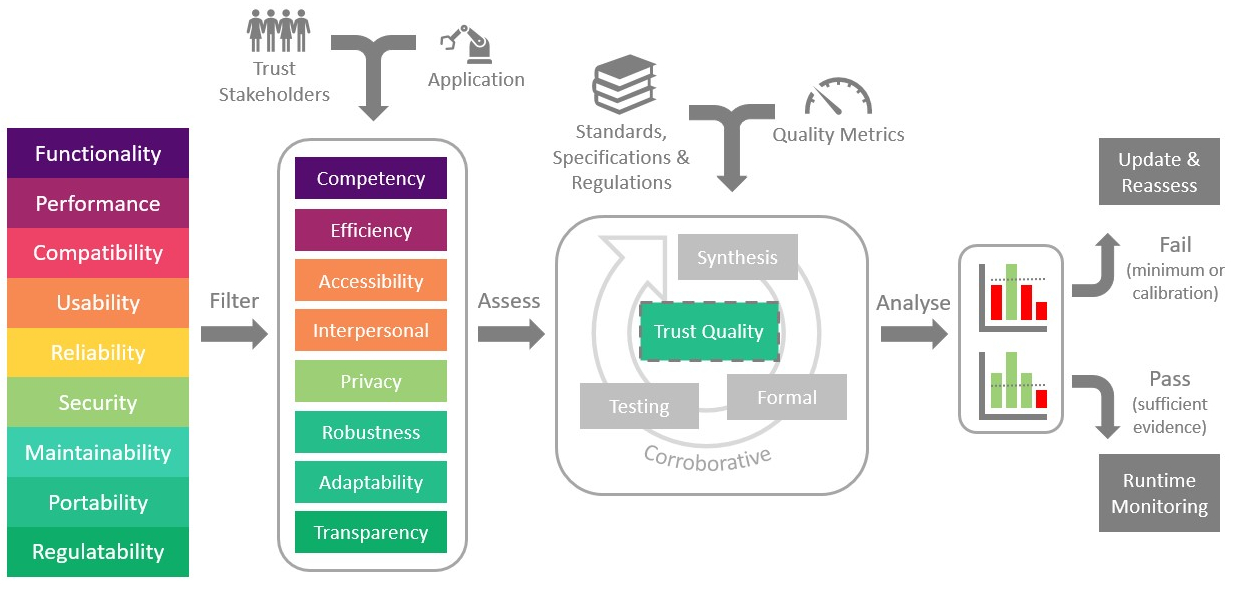
\includegraphics[width=0.98\linewidth]{\pathToOtherFiles/figures/tas_ver.jpg}
    \caption{AS trustworthiness assessment process}
    \label{fig:tas_ver}
\end{figure*}


Further to this issue, are the lack of \emph{standards} against which some trustworthy qualities should be appraised and the \emph{methods} by which they should be evaluated. For example, there are standards for correct road driving conduct~\cite{highwayCode} but no ethical standards by which those driving decisions should be made. 
%
Although headway is being made into developing standards for non-functional properties, such as guidelines for ethical AI [ref EU AI high level expert group] and checklists for HRI best practice ~\cite{kraus2022trustworthy}, there are still areas that need attention, such as standards and specifications for transparency~\cite{winfield2021ieee} and explainability, asethetics and fairness~\cite{Abeywickrama2022}. 
%
Additionally, there is more that can be done at the design stage to improve \emph{verifiability} [add ref]. Evidence for system correctness is essential, but this must be supported with decision explanation~\cite{koopman2018toward}. , whilst maintaining IPR around sensitive hardware and software algorithms [ref]. 



%
To present a defensible safety argument for AS and SCAS...
trust stakeholders
\emph{trust qualities}
application specific
What human factors are considered eg. ISO29119


In addition to assessing the AS trustworthiness, there must also be consideration to gain, calibrate and maintain user trust in the system~\cite{kok2020trust, Chiou2021}, else failures related to overtrust and undertrust are possible. 


%\subsection{Document Structure}
In the following, related work is reviewed in Section


% ****************************************
% ************** Trustworthiness Qualities
% ****************************************

\subsection{Trustworthiness Qualities}

Trust can be expressed in a number of ways and directions; trust the user has in the system, the objective trustworthiness of the system and the context in which the interaction between the two takes place~\cite{Hancock2021}. 
%
In this research we consider the trustworthiness of the system and the specific qualities that must be demonstrated, but we acknowledge the importance of the other mechanisms where human-system trust can be gained or lost in which there has been much contribution from the HRI, psychology and human factors community~\cite{Floridi2019,Lee2004,kok2020trust,Chiou2021,Kohn2021,kraus2022trustworthy}. 
%
Trustworthiness of autonomous systems in the context of this work then, results from objective assessment of the system with respect to a set of appropriate standards. 
%
There has been much academic deliberation on the specific qualities that comprise trustworthiness of AS, specifically for AI~\cite{Thiebes2021,Wing2021} and HRI~\cite{kraus2022trustworthy,atkinson2012trust}
%
Devitt argues that reliability and accuracy are the central pillars of trustworthiness and that other properties stem from these, stating that adaptability and redundancy are higher-order properties of reliability~\cite{devitt2018trustworthiness}. 
%
Thiebes et al. argue for five foundational principles of trustworthy AS (1) beneficence, (2) non-maleficence, (3) autonomy, (4) justice, and (5) explicability~\cite{Thiebes2021}.  


% ****************************************
% *************************** Related Work
% ****************************************
\section{Related Work}\label{Related_work}

Floridi suggests the need for agreed upon metrics for trustworthiness of AI systems and suggests an  AI Trust comparison index, metrics are needed for benchmarking AI suitability to the public.

Rudas and Haidegger also supports the idea of agreed upon metrics from the verification community that can be used to ensure reliability of complex autonomous systems~\cite{Rudas2020}. Wang et al. go further and propose a  theoretical framework of \emph{tripartite trustworthiness} covering; \emph{to-be trust} (trustfulness of an entity or structure), \emph{to-do trust} (trust in an action or behaviour) and \emph{system trust} (a statistical runtime evaluation of performance) and set out 18 formal definitions~\cite{Wang2020}. 



% ****************************************
% ******************* Assessment Framework
% ****************************************
\section{Assessment Framework Vision}\label{Assessment_Framework_Vision}


Below is a checklist for assessemnt of AS trustworthiness:





\noindent\textbf{Verification Methods}: %
Kress-Gazit et al. state that assessment in the correctness of AS can be broken down into four approaches: synthesis of correct-by-construction systems, formal verification at design time, runtime verification or monitoring, and test-based methods~\cite{kress2021formalizing}. 






% ****************************************
% ********************* Existing Standards
% ****************************************

\subsection{Existing Standards for AS}
Existing standards on verification (from Rudas 2020): P1872.1, P2817, P7000 and P7007.

Safety of autonomous systems (from Hawkins 2022): UL4000 [Underwriters Laboratories. Standard for evaluation of autonomous products, 2020] or SCSC-153B [Safety of Autonomous SystemsWorking Group. Safety assurance objectives for autonomous systems, 2022. URL: https://scsc.uk/scsc-153B]


Ethical framework for AI~\cite{Floridi2018} ``offer 20 concrete recommendations to assess, to develop, to incentivise, and to support good AI"

Porter2022 presents an ethical assurance argument for AS, extending the assurance case considered for safety to include ethical standards

devitt2018trustworthiness 

\textcolor{red}{Dhaminda to contribute here?}

\subsection{Future Challenges in Standards}

Riaz et al.~\cite{Riaz2018} suggest the idea of using social norms and human emotions as a standard by which better self-driving controllers may be developed. This idea sets the way for not just development of higher functioning AS, but also standards of trustworthiness by which they can be judged. Although there is much scholarly work on the theory and modelling of social norms, e.g.~\cite{hechter2001social}, there is yet to be published a standard that could be used to objectively assess an autonomous system. 

In some cases, e.g. driving, legislation on appropriate conduct is presented to society in the form of guidelines such as the UKHC in the UK~\cite{highwayCode} but must be translated to a computer readable format to act as an appropriate standard, or set of assertions~\cite{harper2021safety}, if these guidelines can be used to assess AS trustworthiness. A similar process will have to be undertaken for other standards which have yet to be defined, e.g. cooperation, fairness or verifiability, to ensure all aspects of trustworthiness can be assessed. 


% ****************************************
% ********************* Existing Standards
% ****************************************

\subsection{Assessment Methods \& Corroborative Evidence}
Gaining reliability assurance of SCASs using testing alone is unfeasible given the often high-dimensional operational state space. Multiple testing methodologies should be employed where appropriate, e.g. verification, falsification and testing, [Harper Corroborative 2022] combining mutually consistent evidence from multiple and diverse assessment methods will raise the confidence in system trustworthiness.

Knowledge of the internal state of the system is often hidden, e.g. blackbox, due to IP and commercial sensitivity, but whitebox access will be essential for certain aspects of trustworthiness assessment. This may not need to reveal sensitive algorithms but just enough information through observability points in the software architecture could go a long way to understanding if automated decisions are made for the right reason~\cite{koopman2018toward}. 



% ****************************************
% ********************* Existing Standards
% ****************************************

\section{Conclusion}\label{conclusion}






% ***********************************
% ***********************************
% ***********************************
% notes


% \section{Verification for Swarms}\label{sec:verification}

% % Once designed/evolved/implemented with the above considerations it will still be important to test and monitor the resulting behaviours. To do this we can verify etc...
% Verification and validation (V\&V) is the process to gain confidence in the correctness of a system relative to its requirements. Prior to and separate from verification, a specification of the the system must clearly define the expected operational behaviour of the system and many challenges are associated with this task for autonomous systems~\cite{Abeywickrama2022}. There are different verification methods that can be employed and are often chosen relevant to the application, operational domain and the specific properties that need to be verified.

% \subsection{Swarm Trustworthiness Qualities}\label{sec:verification-qualities}
% A swarm must not just be functionally correct but fully trustworthy if it is to integrate with, and be useful to society. Verifying trustworthiness qualities may require methods extending beyond traditional V\&V techniques, as trustworthiness is a meta-property that encapsulates not just safety and functional correctness but many other non-functional attributes, for example, reliability, performance and ethics~\cite{Floridi2019, Wing2021, Lee2004}. A major challenge in verification of these more broad trustworthiness qualities are the lack of standards and regulations by which they can be evaluated against. And whereas verification methods of assessing, for example, functional correctness are relatively mature, there also exists the challenge of devloping robust methodologies for these more nuanced trustworthiness qualities. For example, there are well defined rules for driving conduct and expected behaviour [UKHC] which could be verified using simulation based verification [harper22] but standards for social interaction, aesthetics or ethical behaviour are either non-existent or just emerging [EU directive for AI ethics]. 
% %
% In addition to assessing the trustworthiness of the swarm, there must also be consideration to gain, calibrate and maintain user trust in the system~\cite{Chiou2021}, as under- or overtrust in the system can lead to serious and sometimes fatal consequences~\cite{kok2020trust}.

% \subsection{Swarm Trustworthiness Qualities \& Assessment}\label{sec:verification-qualities-swarm}
% Robustness, scalability and adaptability are considered as being particularly useful qualities of swarm trustworthiness, although this list could be extended to cover many other trustworthy qualities [https://github.com/TSL-UOB/TAS-Verif]. 
% %
% \subsubsection{Trust Quality: Robustness}
% Robustness is the degree to which the system can function correctly in the presence of invalid inputs or stressful conditions~\cite{ISO24765}. For a swarm application invalid or stressful inputs could be, for example, individual agents failing, poor environmental illumination or limited network connectivity. \textcolor{red}{JAMES - are there other robustness factors to consider here for swarms?}. 
% %
% A suitable verification task may be to find the limits of robustness either through simulation and/or physical trials of task success to ensure that this meets the specifications. 
% %
% A swarm system operating in a bound environment with a fixed number of allowable agent actions is a relatively constrained problem compared to, say, a self-driving vehicle. A swarm that chooses from a fixed set of actions (e.g. behaviour tree) is well suited to verification via formal modelling. 
% %



% \subsubsection{Trust Quality: Scalability}
% Scalability is defined as...How do autonomous systems (swarms) of increasing scales affect trust? \textcolor{red}{JAMES - my interpretation of scalability would be how well/easily can the system be operated at a larger size. Increasing the size could impact on other functional and non-functional requirements, e.g. box delivery rate, collision frequency, user acceptance. Are you intending to explore the knock-on/secondary effects or was there something specific to size you wanted to explore?}. Trustworthy scalability metrics could comprise performance analysis give a change in swarm scale, usability of the swarm given the larger size and safety properties concerning collisions (tbd with James). 

% \subsubsection{Trust Quality: Adaptability}
% Adaptability is the degree to which a system can effectively and efficiently be adapted for different or evolving hardware, software or other operational or usage environments~\cite{ISO24765}. For a swarm application, this could be operating well with environmental obstructions, e.g. blocked path in a warehouse and having to find another route. In this case effective trustworthy metrics could be based around agent idle times (time not spent doing something useful) and recovery rates (speed at which a new route is found) when the swarm encounters a blocked paths. Additionally application performance metrics could be used to assess adaptability of swarms, for example task success rates in a find-and-fetch operation could be used for the swarm in a new building layout.

% \subsubsection{Trustworthiness of Emergent Behaviour}
% \textcolor{red}{Do we need to say here about emergent behaviours that cannot be assessed at the agent level? Or are we steering clear?}
% %
% \subsection{Trustworthiness Assessment Methods}\label{sec:verification-qualities-methods}
% Different verification methods will be more or less suitable to different domains based on the application. 
% %
% Formal verification requires a model of the system written in a formal language and can be used to prove a system (e.g. swarm) property is consistent against an \emph{entire} parameter space. This is in contrast to \emph{sampling} the parameter space if using a testing method, e.g. simulation technique. Formal verification provides a proof of assurance against single properties but the model generation can be non-trivial and the technique is not always suitable for complex systems operating in unbound domains, i.e. high dimensional parameter space. 
% %
% However, a swarm system operating in a bound environment with a fixed number of allowable agent actions is a constrained problem relative to, say, a self-driving vehicle. A swarm of robot agents that use a fixed set of actions (e.g. behaviour tree) is exactly suited to verification via formal model. 
% %
% Formal methods have been demonstrated to show robustness of a swarm to network connectivity loss using probabilistic finite state machine (PFSM) verification~\cite{Winfield2008} and is a valid method for this application. 
% %
% Although formal models can give assurance against an entire range of parameters, a drawback is that only gives assurance of the \emph{model} and there may be distinct difference between the model and the real system. This is where \emph{testing} methods, such as simulation based verification, can fill the gap. 

% % Testing-based methods can be used in a complementary and even corroborative manner to support a formal analysis. Corroborative V\&V seeks to combine mutually consistent evidence from multiple and diverse assessment methods will raise the confidence in system trustworthiness~\cite{harperFMAS22}. Physical and Simulation-based verification methods execute a single test case where a single output will be monitored as a pass or fail, and multiple test cases are used to build a \emph{test suite}. Testing techniques therefore rely heavily on test generation to produce a diverse and challenging test suite, a set of stimulus that will complement any formal assessment but also test any model assumptions and the bounds of the operational domain (edge cases). 

% Many techniques can be employed to build a suitably diverse test suite~\cite{MarkUtting2012} including; random test generation, manually written test cases (based on historical evidence or accidentology), fault-based test selection, requirements coverage based and agent-based~\cite{chance2020agency}. 
% %
% There are also assertion-based techniques that can be used to prove that the system complies with a set of provided rules, e.g. diving conduct for self-driving vehicles~\cite{harper2021safety}. 

% Runtime verification techniques can also be utilised as a post-design strategy to trustworthiness assurance, where an oracle is used to compare current and expected behaviour~\cite{Leucker2009}. Runtime verification requires a suitable oracle to be defined which sets the expected bounds of operation, similar to a pattern-of-life model, and can be useful for complex systems where exhaustive design-time verification is intractable and if the system can be expected to change regularly, e.g. software updates pushed regularly without time for a complete system re-verification. 

% % ******************** TODO
% Verification of the trust qualities of robustness, scalability and adaptability for a swarm are suited to a mix of formal and testing-based verification. A PFSM approach could be suitable to prove system robustness to network connectivity and task completion rate~\cite{Winfield2008}. Complementary to this, simulation should be used for assertion-based analysis of the system relative to the requirements, to ensure the system behaves as specified. 
% %
% Additionally, simulation may be used for capturing scalability information by increasing the swarm size, and reliability information compiled from long horizon observations. 
% %
% Where long-horizon testing is not feasible but high reliability is needed for low probability faults, e.g. safety critical aspects of the system, then reliability models can be used to estimate future fault rates that can be assessed against a specified \emph{fault tolerance level}~\cite{Butler1993}. 
% % Arguments of high reliability often assume that isolated components fail independently which is a parallel that can be drawn to a swarm of individual robot agents. 
% %
% Physical testing should be done to validate formal and simulation-based methods and potentially explore scenarios not possible in either of the non-physical methods. As physical testing is usually the more costly method, a test plan should set out and prioritise the most important trust qualities to analyse, e.g. safety-critical testing may be a priority. Validation of simulated results will help to build a strong and corroborative argument of swarm trustworthiness.
\balance

% ***************************************************
%  Bib
% ***************************************************
\printbibliography

% ***************************************************
%  Appendix
% ***************************************************
% % \newpage
% \begingroup
% \let\clearpage\relax 
% \onecolumn 
% % \newpage
% \section*{Appendix A}\label{appendix_a}
% Figure \ref{fig:overtaking_analysis_diag} presents a model of an overtaking manoeuvre, showing the derivation of a formula for calculating Safe Distance Ahead, which was used in the simulation study results presented in Section \ref{sim_case_study}.
% \begin{figure*}[h]
% %    \centering
%     \includegraphics[width=18cm]{../other/figures/Overtaking_Manoeuvre_Analysis_global_view_v2.png}
%     \caption{Schematic of Model-based Analysis of Overtaking Manoeuvre.}
%     \label{fig:overtaking_analysis_diag}
% \end{figure*}
% \endgroup

\end{document}
% \grid
